\documentclass[10pt]{exam}
\usepackage[hon]{template-for-exam}
\usepackage{tikz,graphicx,multicol}
\usetikzlibrary{shadings,decorations.pathmorphing}

\tikzstyle{vector}=[
  ->,
  red,
  thick
]

\title{Relative Velocity}
\author{Rohrbach}
\date{\today}

\begin{document}
\maketitle



\begin{align*}
  \vec{v}_{AC} &= \vec{v}_{AB} + \vec{v}_{BC} &
  \vec{v}_{AB} &= -\vec{v}_{BA}
\end{align*}


\begin{questions}

\question
  A motor boat travels at a velocity 7 m/s north (with respect to the water).  The river flows north at a speed of 3 m/s (with respect to the shore).  From the perspective of someone standing on the shore, what is the boat's velocity?


  \begin{center}
    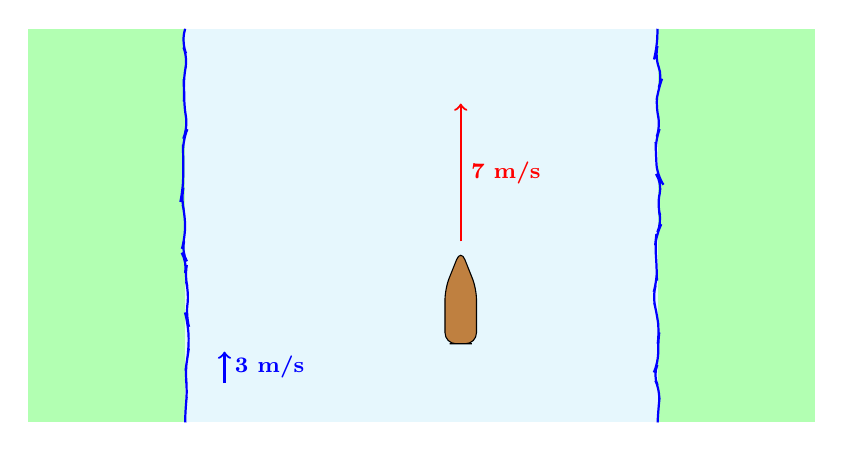
\begin{tikzpicture}
      \begin{scope}
        \tikzstyle{riverbank}=[
          blue, thick, 
          decorate, 
          decoration={
            random steps,
            segment length=2mm,
            amplitude=2pt
          },
          rounded corners
        ]
        \tikzstyle{water}=[
          blue, thin, 
          decorate, 
          decoration={
            random steps,
            segment length=2mm,
            amplitude=2pt
          },
          rounded corners
        ]
        \fill[green!30] (-1,-1) rectangle ++ (-2,5);
        \fill[green!30] (5,-1) rectangle ++ (2,5);
        \fill[cyan!10] (-1,-1) rectangle ++ (6,5);
        \draw[riverbank]
          (-1,-1) -- ++(0,5);
        \draw[riverbank] (5,-1) -- ++(0,5);
        \draw[vector,blue] (-0.5,-0.5)
          -- ++(0,0.4) node[midway,right] 
          {\footnotesize \bf 3 m/s};
      \end{scope}
      \begin{scope}[rounded corners, rotate=90]
        \draw[fill=brown] (0,-2.5)
          -- ++(0,.2)
          -- ++(.7,0)
          -- ++(.5,-.2) coordinate (boat front)
          -- ++(-.5,-.2)
          -- ++(-.7,0)
          -- cycle;
      \end{scope}
      \draw[vector] 
        (boat front) ++(0,0.1) -- ++(0,1.75)
        node[midway, right] 
          {\footnotesize \bf 7 m/s};
    \end{tikzpicture}
  \end{center}

  \vs

  \question
  A motor boat travels at a velocity 7 m/s {\bf south} (with respect to the water).  The river flows north at a speed of 3 m/s (with respect to the shore).  From the perspective of someone standing on the shore, what is the boat's velocity?


  \begin{center}
    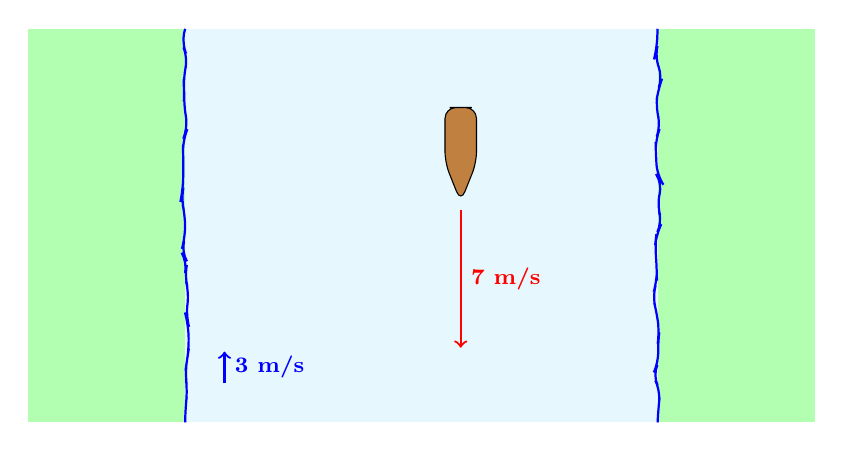
\begin{tikzpicture}
      \begin{scope}
        \tikzstyle{riverbank}=[
          blue, thick, 
          decorate, 
          decoration={
            random steps,
            segment length=2mm,
            amplitude=2pt
          },
          rounded corners
        ]
        \tikzstyle{water}=[
          blue, thin, 
          decorate, 
          decoration={
            random steps,
            segment length=2mm,
            amplitude=2pt
          },
          rounded corners
        ]
        \fill[green!30] (-1,-1) rectangle ++ (-2,5);
        \fill[green!30] (5,-1) rectangle ++ (2,5);
        \fill[cyan!10] (-1,-1) rectangle ++ (6,5);
        \draw[riverbank]
          (-1,-1) -- ++(0,5);
        \draw[riverbank] (5,-1) -- ++(0,5);
        \draw[vector,blue] (-0.5,-0.5)
          -- ++(0,0.4) node[midway,right] 
          {\footnotesize \bf 3 m/s};
      \end{scope}
      \begin{scope}[rounded corners, rotate=-90, shift={(-3,0)}]
        \draw[fill=brown] (0,2.5)
          -- ++(0,.2)
          -- ++(.7,0)
          -- ++(.5,-.2) coordinate (boat front)
          -- ++(-.5,-.2)
          -- ++(-.7,0)
          -- cycle;
      \end{scope}
      \draw[vector] 
        (boat front) ++(0,-0.1) -- ++(0,-1.75)
        node[midway, right] 
          {\footnotesize \bf 7 m/s};
    \end{tikzpicture}
  \end{center}

  \vs


\pagebreak



\question
  A motor boat travels at a velocity 7 m/s {\bf east} (with respect to the water).  The river flows north at a speed of 3 m/s (with respect to the shore).  From the perspective of someone standing on the shore, what is the boat's velocity (magnitude and direction)?


  \begin{center}
    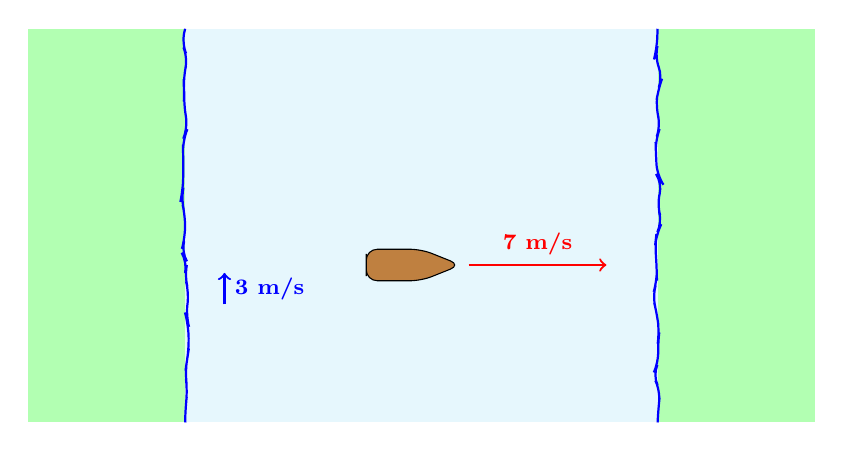
\begin{tikzpicture}
      \begin{scope}
        \tikzstyle{riverbank}=[
          blue, thick, 
          decorate, 
          decoration={
            random steps,
            segment length=2mm,
            amplitude=2pt
          },
          rounded corners
        ]
        \tikzstyle{water}=[
          blue, thin, 
          decorate, 
          decoration={
            random steps,
            segment length=2mm,
            amplitude=2pt
          },
          rounded corners
        ]
        \fill[green!30] (-1,-2) rectangle ++ (-2,5);
        \fill[green!30] (5,-2) rectangle ++ (2,5);
        \fill[cyan!10] (-1,-2) rectangle ++ (6,5);
        \draw[riverbank]
          (-1,-2) -- ++(0,5);
        \draw[riverbank] (5,-2) -- ++(0,5);
        \draw[vector,blue] (-0.5,-0.5)
          -- ++(0,0.4) node[midway,right] 
          {\footnotesize \bf 3 m/s};
      \end{scope}
      \begin{scope}[rounded corners]
        \draw[fill=brown] (1.3,0)
          -- ++(0,.2)
          -- ++(.7,0)
          -- ++(.5,-.2) coordinate (boat front)
          -- ++(-.5,-.2)
          -- ++(-.7,0)
          -- cycle;
      \end{scope}
      \draw[vector] 
        (boat front) ++(0.1,0) -- ++(1.75,0)
        node[midway, above] 
          {\footnotesize \bf 7 m/s};
    \end{tikzpicture}
  \end{center}

  \vs

  \question
  Car \#1 is going 80 MPH east.   Car \#2 is going 56 MPH east.  From the perspective of Car \#1, what velocity does Car \#2 have?
  \vs
  





\end{questions}

\end{document}